%%%%%%%%%%%%%%%%%%%%%%%%%%%%%%%%%%%%%
Memorization is a phenomenon where machine learning models, particularly deep neural networks, retain information about specific training examples instead of learning patterns that generalize well to unseen data.This concept is crucial in understanding the behaviour of the model, especially in the context of overfitting, where a model achieves high accuracy   on training data but performs poorly on the test set. The high capacity and complex parameter space of deep neural networks enable these models to store detailed information from individual training samples, which causes poor generalisation and makes them susceptible to capturing noise rather than robust, transferable features \cite{ali_raza_537a9747}. 

Researchers have further refined the concept of memorisation,  often distinguishing mainly between Memorization Learning , which refers to the process of learning specific details or particular features of examples, and Pattern Learning which focuses in on extracting common patterns or generalised features  in the data \cite{jiaheng_wei_8cfd95ec}. Understanding the distinction is crucial for diagnosing model’s behaviour, and developing explanaible AI systems that can reveal whether a  model’ decision is driven by the memorisation or meaningful, generalisable patterns. 

The following subsections expand on these ideas: Conceptual Deepening,  provides the theoretical and mathematical background of Memorization giving ; Generalisation Tradeoff which examines the distinction between Generalisation vs. Memorisation;Memorisation in Convolutional Neural Networks  examines the reason why CNNs are particularly prone to memorisation; and  Mitigation Techniques for Memorization survey the methods to reduce memorization in deep learning models.
%%%%%%%%%%%%%%%%%%%%%%%%%%%%%%%%%%%%%
\subsubsection{Conceptual Deepening of Memorization}
Memorization refers to the ability of model’s parameters to store and recall specific training examples rather than learning underlying data distributions. The traditional view of generalization posits that deep neural networks due to their over-parameterized, complex structure results in overfitting the training set yields poor generalization to validation set and test sets \cite{ian_goodfellow_5e6a80c8}. However , empirical evidence shows that deep neural networks often achieve excellent generalisation performance , ‘well’ accuracy score with sufficient capacity \cite{devansh_arpit_9e68508c}. \cite{chiyuan_zhang_bd8f0549} highlight a remarkable property of deep neural networks: despite achieving zero training error, implies overfitting, these models can still maintain low test error. The real question is how these models achieves this state-of-art conditions? \cite{chiyuan_zhang_bd8f0549}furthers this question by varying experimental conditions on neural networks ,examining how generalization performance changes under data corruptions and label corruptions on CIFAR-10.  Importantly ,even when the corruption destroys the relationship between images and labels, networks learning capability slows down yet neural networks are still able to fit  the training data perfectly. 
- Burda generalization error formulayi ver
Furthermore, this experiment highlights the rising testing error under the data corruption, emphasizing that there is a strong memorization capability. These oservations could not able to explain with a statistical learning theory where we imply different complexity measures, controlling generalisation error. These include VC Dimension \cite{vladimir_vapnik_d1c1a1dc}, which quantifies the complexity of a hypothesis space independently of the underlying data distribution; and its pseudo-dimension. Rademacher complexity \cite{shai_shalev_shwartz_c0318cbc}, refines VC Dimension including distribution dependent complexity that naturally apply to real-valued  and multi-class function classes. Finally, Uniform stability measures the sensitivity of a learning algorithm to small perturbations in the training set.
The observed distinction between generalization and memorization underscores that achieving low training error do not necessarily imply that meaningful patterns have been learned. Classical complexity measures alone appear insufficient to fully explain this paradox. To explain memorization beyond classical complexity measures, it is essential to examine the nature of the information being retained. Specifically, recent literature distinguishes between two fundamental mechanisms: label memorization and feature memorization. 
\paragraph{Label versus Feature Memorization}
Label Memorization refers to the phenomenon where models memorize the labels in training datasets without learning the relevant patterns that the label can be predicted . This propensity for label memorization, cannot be explained by the classical generalization formula , which is the sum of the empirical error in training set and the generalization gap controlled by the model complexity parameter and the empirical error.  \cite{chiyuan_zhang_bd8f0549}, conducted experiments demonstrating the label memorization phenomenon on CIFAR-10. Their results show that, models trained on datasets with random labels achieve almost  zero-training error, while experiencing severe generalization degradation. Specifically, they observed that as label corruption increases 0\% to 100\%, the convergence increases significantly, yet models continue to memorize the corrupted labels, resulting in high  generalization error (since the training error is 0). 
In contrast, feature memorization involves the model learning and retaining spurious features that are uncorrelated with the true underlying data distribution.\cite{simone_bombari_23e6de9b} \cite{yang_yu_4720d432} This type of memorization, stated in (Yu et al., 2023) , is separable based on the model’s output early in training. In the experiment, a colored MNSIT used as an example of spurious correlations. Each digit in MNSIT datasets is a class , where the majority of digits have a particular color, and the remaining digits are in other colors. The model, therefore, learn to associate the color with the core feature instead of the digit’s shape, leading to poor generalization on correlations where the spurious correlation between color and digit is broken \cite{chenyu_you_e79f4b0f}.  While feature memorization describes the model’s propensity for learning uncorrelated patters, a closely related phenomenon known as Shortcut Learning explains the mechanism behind this behaviour.
\paragraph{Shortcut Learning and its Implications}
Shortcut Learning in neural networks, occurs when a model achieves high performance on a standard benchmark, not by comprehending the underlying data correlations between input and output, but using shortcut features or exploiting trivial associations that fail in generalization performance \cite{robert_geirhos_e33ec72d}.  As an example , a model trained to distinguish between wolves and huskies might learn to associate snow in the background with wolves, rather than focusing on the animals' distinct facial features \cite{chenyu_you_e79f4b0f}. Another example is provided in (Geirhos et al., 2020) an image classification task where the model is trained to identify stars and moons , instead of learning the actual shape of the  objects , it exploit the location of the images .This indicates that the model has learned a “shortcut”- a decision rule that performs well on training distribution but fails in generalization tests. 

This phenomenon has serious implications in applications requiring robustness and fairness . In the article \cite{joy_buolamwini_0378cfd5} conducted an experiment over the 3 different parliamentary benchmarks  to illustrate the social amplification on neural networks. Given benchmarks were IJB-A US Government Benchmark published by NIST ( National Institute of Standards and Technology) in 2015 and Adience is a widely-used face image dataset originally developed for gender and age classification; yet these models overrepresented lighter males, underrepresented darker females, thereby underrepresented of darker individuals in general. PPB ( Pilot Parliaments Benchmark) was therefore focused on achieving better intersectional representation  in balanced datasets. To provide a comprehensive evaluation of these biases in real world applications; examined three commercial gender classification systems: Microsoft, IBM, and Face++. These classifiers were selected because they represented the state-of-the-art in facial analysis technology and were widely deployed in commercial products during that period of time. The result demonstrates that even with a balanced representation of protected characteristics, models may still exhibit bias amplification in darker-skinned people. Especially the highest error rates  were observed for darker-skinned females ranging from 23.8\% for Microsoft to 36.0\% for Face++ and 33.1\% for IBM \cite{anoop_krishnan_6fbfbe57}. The underlying cause is that the models tend to learn the shortcut way ,  relying on “facial geometries” and “gender norms“ specific to the majority group of population in the training set, failing to generalize to minority subgroups.

When a model’s decision boundary is defined by memorized shortcuts rather than learning robust semantic representations, it becomes vulnerable to critical security issues. In the following section , memorization based fragility is targeted through white-box adversarial attacks, specifically focusing on the mechanisms of FGSM and PGD.
\begin{table}
    \centering
    \begin{tabularx}{\textwidth}{|X|X|X|X|X|X|X|X|X|X|}
    \toprule
    \multicolumn{10}{|c|}{\textbf{Dataset Properties Comparison between Benchmarks}} \\
    \midrule{}
    \textbf{Dataset} & \textbf{n} & \textbf{Female} & \textbf{Male} & \textbf{Darker} & \textbf{Lighter} & \textbf{DF} & \textbf{DM} & \textbf{LF} & \textbf{LM} \\
    \midrule{}
 PPB   & 1270  & 44.6\% & 55.4\% & 46.4\% &53.6\% & 21.3\% & 25.0\% & 23.3\% & 30.3 \%\\
 IJB-A & 500  & 24.6\% & 75.4\% & 20.4\% & 79.6\% & 4.4\% & 16.0\% & 20.2 \% & 59.4 \%\\
 Adience & 2284 & 52.0\% & 48.0\% & 13.8\% & 86.2\% & 7.4\% & 6.4\% & 44.6\% & 41.6 \% \\

 \bottomrule
\end{tabularx}



\end{table}
%%%%%%%%%%%%%%%%%%%%%%%%%%%%%%%%%%%%%
\subsubsection{White-Box Attacks in DNN and Its Correlation with Memorization }
To evaluate the security implications of memorization, this section focuses on White-Box attacks. Unlike Black-Box scenarios where the attackers could not have any knowledge of the internal architecture, parameters or training data of the model, White-Box scenarios allows studying memorization by examining model’s vulnerabilities, specifically “jagged” points where the model can be systematically exploited. To understand these vulnerabilities, the adversarial space should be defined. Adversarial Space according to \cite{chio_clarence_9b691fc0}, is a result of imperfect representation in training data where the entire input space cannot be provided . This imperfect representation of the input space provided in training data in white-box models , allows Attackers exploiting “Sensitivity” of memorized features  and moving the direction that the model is “weakest”. In standard training , gradient-descent is utilized as an  optimization algorithm to minimize the cost function by updating model weights , attackers used the transparency of white-box models to reverse this logic. Instead of updating weights to minimize loss, they keep the weights fixed and perturb the input pixels to maximize the loss function. To illustrate this phenomenon , we will examine two primary gradient-based strategies: Fast Gradient Sign Method( FGSM) and Projected Gradient Descent (PGD).
\paragraph{Fast Gradient Sign Method (FGSM)}
The Fast Gradient Sign Method (FGSM) , introduced in  \cite{ian_goodfellow_5e6a80c8} adding subtle perturbations into the gradient of the cost function with respect to the original input to maximize the misclassification and thereby highlighting vulnerabilities in deep learning networks. Specifically, the sign of the gradient indicates the direction in which the input pixels must be altered to increase the loss function J. By moving the input in this direction by a small step ϵ, FGSM creates an adversarial image xadv that is often indistinguishable from the original image without visible changes but results in incorrect classification by the model.  A key theoretical insight behind FGSM, is that neural networks are too linear to resist linear adversarial perturbations \cite{ian_goodfellow_5e6a80c8} . Components such as ReLU and maxout networks are intentionally designed to behave linearly to facilitate easier optimization during training. As a consequence, the cumulative effect of a small change in each input dimension results in a drastic change in the final output. FGSM exploits this linearity ; the attacker moves the input across the sign of the gradient with minimal computational effort, making it one of the most efficient adversarial attack strategies. This is empricaly demonstrated in “ panda vs. gibbon” example , where a perturbation of merely  ϵ= 0.007 is sufficient to cause misclassification.
\begin{figure}[ht]
    \centering
    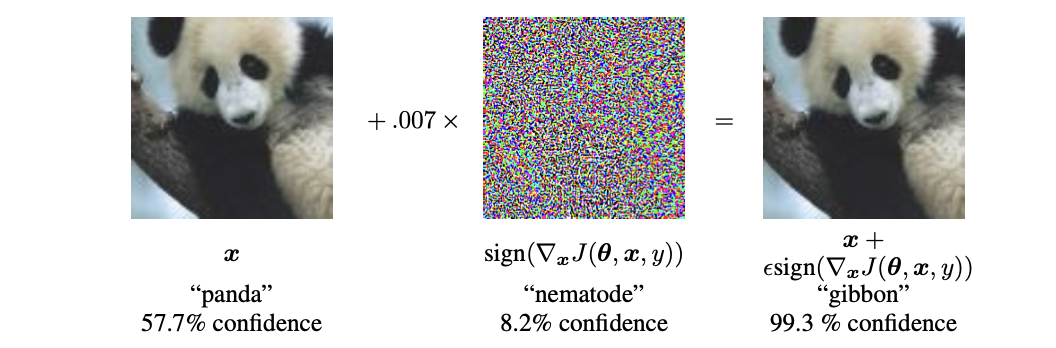
\includegraphics[width=0.8\textwidth]{figures/fgsm.png}
    \caption{Adversarial Example Generated by FGSM}
    \label{fig:panda}
\end{figure}
As discussed , the adversarial space emerges from the imperfect representation of the input space during training. Memorization amplifies this imperfections by increasing the model’s susceptibility to gradient-based perturbations. When a model prioritizes memorizing specific samples over learning generalizable features, the resulting decision boundaries become highly “jagged” and fragile. These boundaries narrow the distance between training data, which attackers can systematically exploit using fast gradient sign method to shift  the input into incorrect classification zone. 
\paragraph{Projected Gradient Descent (PGD)}
While FGSM provides single-step attacks , PGD provides iterative approach by applying small perturbations to the input data to maximize the model’s prediction error. Based on the information given in \cite{aleksander_m_dry_8d27e246}, the inner problem is to find a perturbation that causes the greatest increase in loss function. In prior studies , the linearization approach that is used in FGSM , a single step approach , is not enough to understand the inner problem in more detail. The iterative nature of PGD allows for a more exhaustive search for adversarial examples repeatedly applying first-order gradients to navigate the complex loss landscape. In the experiment provided in \cite{aleksander_m_dry_8d27e246}, states that given datasets of MNSIT and CIFAR-10 , the adjusted PGD attack consistently outperformed FGSM in terms of attack success, with a higher percentage  of loss maximization with CIFAR-10 dataset. Even though MNSIT and CIFAR-10 are robust to adversarial attacks, MNSIT achieves high accuracy for wide range of powerful ℓ∞-bound adversaries and large perturbations due to the large fraction of atypical samples contained in CIFAR-10 .

Furthermore, Memorization amplifies the effectiveness of PGD by exploiting the model’s vulnerabilities in training by generating a very jagged loss landscape. While PGD is a first-order (gradient-based) adversary, if the gradients are “shattered“ or “noisy“ due to memorization, PGD might get stuck in poor local maximum, making the model appear  robust when it actually isn’t.

\clearpage
%%%%%%%%%%%%%%%%%%%%%%%%%%%%%%%%%%%%%

